\anonsection{Задание лабораторной работы}
На основе своего варианта задания рассчитать количество функциональных точек для разрабатываемого программного приложения. 
С этой целью разработать программный инструмент.
Произвести оценку трудозатрат и длительности разработки по методике COCOMO II с использованием моделей композиции приложения и ранней разработки архитектуры.
Определить среднюю численность команды разработчиков.
На основе экспертной оценки стоимости человеко-месяца произвести предварительную оценку бюджета проекта.
Дать заключение о применимости метода функциональных точек и модели COCOMO II, а также их сравнение с базовой моделью СОСОМО для решения поставленной задачи с учетом своего варианта.


\anonsection{Условие лабораторной работы по варианту} 
Компания получила заказ на разработку клиентского мобильного приложения брокерской системы. 
Программа позволяет просматривать актуальную биржевую информацию, производить сделки и отслеживать их выполнение.
Приложение имеет 4 страницы: авторизация, биржевые сводки, заявки, новая заявка.

\subsection*{Авторизация}
На данной странице осуществляется ввод логина и пароля пользователя для входа в систему.
Страница содержит два поля ввода и одну командную кнопку, а также флажок-переключатель, который активируется при необходимости запоминания параметров авторизации.

\subsection*{Биржевые сводки}
Биржевые сводки отражают текущую ситуацию на бирже. 
Страница содержит таблицу, кнопку «Добавить» и диалоговое окно с одним полем для ввода и двумя командными кнопками.

Таблица содержит три колонки: Ценная бумага (имя бумаги), Цена (цена за одну ценную бумагу), Изменение (изменение цены бумаги со времени последнего закрытия биржи). 
Кнопка «Добавить» вызывает диалоговое окно для добавления новой бумаги (окно состоит из поля ввода и кнопок ОК, Cancel).

\subsection*{Заявки}
Заявки содержат таблицу, отображающую текущие (еще не выполненные) заявки на покупку или продажу ценных бумаг.
Таблица содержит четыре поля: Тип (покупка/продажа), Имя бумаги, Цена по которой готовы покупаться/продаваться бумаги, Количество бумаг для покупки/продажи.
При нажатии на любую строку таблицы появляется контекстное меню с возможностью удалить или изменить заявку.

\subsection*{Новая заявка}
Страница позволяет оформить заявку на покупку или продажу ценной бумаги. 
Страница состоит из 4 полей: Бумага (имя бумаги), Цена (цена по которой необходимо купить/продать бумагу), Покупка (булева переменная в
значение true обозначает покупку, false – продажа) и кнопки «Оформить» - для подтверждения оформления заявки.

\newpage
\subsection*{Характеристики продукта}
Разработанное ПО состоит из трех компонентов. 
Первый компонент составляет по объему примерно 15\% программного кода и будет написан на SQL, второй (около 60\% кода) - на С\#, а третий в объеме 25\% кода - на Java. 

\begin{enumerate}
	\item Обмен данными -- 5 (Несколько внешних интерфейсов, несколько типов коммуникационных протоколов).
	\item Распределенная обработка -- 5 (Динамическое выполнение процессов в любом подходящем компоненте системы).
	\item Производительность -- 3 (Время реакции или пропускная способность являются критическими в обычное рабочее
	время. Время обработки ограничено взаимодействующими системами.).
	\item Эксплуатационные ограничения по аппаратным ресурсам -- 2 (Должны учитываться некоторые ограничения, связанные c безопасностью или временем реакции).
	\item Транзакционная нагрузка -- 3 (Ожидаются ежедневные пиковые периоды).
	\item Интенсивность взаимодействия с пользователем (оперативный ввод данных) -- 4 (От 24\% до 30\% транзакций требуют интерактивного ввода данных).
	\item Эргономические характеристики, влияющие на эффективность работы конечных пользователей -- 1 (От одной до трех функциональных возможностей).
	\item Оперативное обновление -- 4 (Онлайновое обновление основных внутренних логических файлов + необходимость специальной защиты от потери данных).
	\item Сложность обработки -- 4.
	\item Повторное использование -- 0 (Отсутствует).
	\item Легкость инсталляции -- 1 (Для установки требуется специальная процедура).
	\item Легкость эксплуатации/администрирования -- 2.
	\item Портативность -- -- 2 (Приложение рассчитано на много установок для строго стандартной платформы (технические средства + программное обеспечение)).
	\item Гибкость -- 2.
\end{enumerate}

Для реализации проекта была сформирована новая команда разработчиков, у отдельных членов которой имеется некоторый опыт создания систем подобного типа. 
В целях сплочения команды были проведены определенные мероприятия, что обеспечило на старте проекта приемлемую коммуникацию внутри коллектива. 
Заказчик не настаивает на жесткой регламентации процесса, однако график реализации проекта довольно жесткий. 
Несмотря на то, что предметная область является для разработчиков относительно новой, анализу архитектурных рисков было уделено лишь некоторое внимание. 
Организация только начинает внедрять методы управления проектами и формальные методы оценки качества процесса разработки.

Надежность и уровень сложности (RCPX) разрабатываемой системы оцениваются как очень высокие, повторного использования компонентов не
предусматривается (RUSE). 
Возможности персонала (PERS) – средние, его  опыт работы в разработке систем подобного типа (PREX) низкий. 
Сложность платформы (PDIF) высокая. 
Разработка предусматривает очень интенсивное использование инструментальных средств поддержки (FCIL). 
Заказчик настаивает на жестком графике (SCED).

\anonsection{COCOMO II}
Модель COCOMO I основана на модели разработки Waterfall, но из-за освоения объектно-ориентированного подхода в процессе разработки программного обеспечения COCOMO I не дает точных результатов. 
COCOMO II позволяет учесть это при разработке проекта.
Первоочередной целью модели COCOMO II является создание возможностей поддержки для постоянного внесения поправок в модель и предоставление количественной аналитической структуры, методов и инструментов. 
Он также способен исследовать влияние усовершенствований программных технологий на жизненный цикл разработки программного обеспечения.
Модели оценки, включенные в COCOMO II, включают модель композиции приложения, модель раннего проектирования, модель повторного
использования и модель постархитектуры.

\subsection*{Модель композиции приложения}
Эта модель предназначена для использования с повторно используемыми компонентами и генерирует оценки разработки прототипа и работает на основе точек объекта.
Модель больше подходит для разработки прототипа системы. 
Чтобы оценить общие усилия, выполняются следующие шаги.

\subsection*{Ранняя модель дизайна}
Модель, используемая на этапе проектирования системы после получения требований. 
Его оценки создаются на основе функциональных точек, которые затем переводятся в несколько строк исходного кода. 

\subsection*{Модель повторного использования}
Это модель, которая вычисляет трудозатраты, необходимые для объединения повторно используемых компонентов или программного кода, который спонтанно создается инструментами проектирования или преобразования программ. 
Есть два типа повторно используемых кодов: черный ящик и код белого ящика. 
Код черного ящика используется, когда в нем нет понимания кода и модификации. 
И наоборот, белое поле используется при интеграции нового кода. 

\anonsection{Реализация приложения}
Для подсчета параметров проекта по методике COCOMO II было реализовано приложение.
В нем можно рассчитать необходимые параметры в четырех вкладках.
В каждом из экранов можно установить необходимые параметры по варианту.

На рисунке представлен вид приложения:
\FloatBarrier
\begin{figure}[h]	
	\begin{center}
		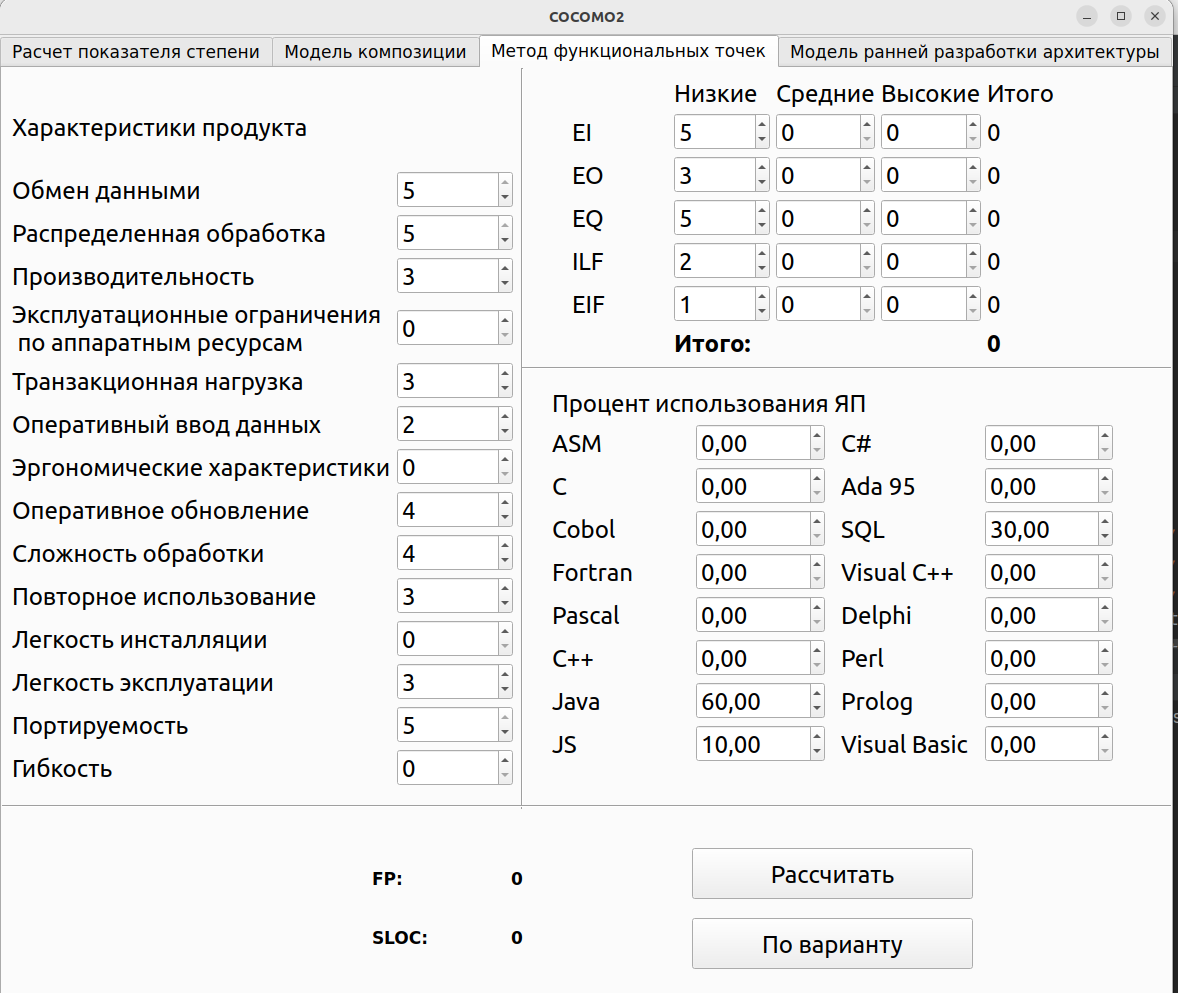
\includegraphics[width=\linewidth]{inc/res.png}
	\end{center}
	\captionsetup{justification=centering}
	\caption{Основной экран приложения}
\end{figure}
\FloatBarrier 

\anonsection{Метод функциональных точек}
Пройдемся по основным параметрам, которые нужно оценить:
\begin{enumerate}
	\item \textit{FTR} -- количество связанных с каждым функциональным типом файлов типа ссылок.
	\item \textit{DET} -- количество связанных с каждым функциональным типом элементарных данных.
	\item \textit{RET} -- количество типов элементов записей.
	\item \textit{EI} -- элементарный процесс, перемещающий данные из внешней среды в приложение.
	\item \textit{EO} -- элементарный процесс, перемещающий данные, вычисленные в приложении, во внешнюю среду.
	\item \textit{EQ} -- элементарный процесс, состоящий из комбинации «запрос/ответ», не связанный с вычислением производных данных или	обновлением внутренних логических файлов (базы данных).
	\item \textit{ILF} -- выделяемые пользователем логически связанные группы данных или блоки управляющей информации, которые поддерживаются внутри продукта и обслуживаются через внешние вводы.
	\item \textit{EIF} --  выделяемые пользователем логически связанные группы данных или блоки управляющей информации, на которые ссылается продукт, но которые поддерживаются вне продукта.
\end{enumerate}

В нашем приложении используются 3 внутренних файла:
\begin{itemize}
	\item таблица с логинами и паролями;
	\item таблица с подробной информации о заявке: ее тип, имя бумаги, цена и количества;
	\item таблица с информацией о бумагах.
\end{itemize} 

Также существует одна внешняя таблица с информацией о бирже с названием бумаги, ценой и изменением.

Вычислим все EI:
\begin{enumerate}
	\item \textbf{Добавить заявку}: одна ссылка на файл ($FTR = 1$), 5 элементов -- (4 поля ввода + кнопка). Уровень сложности -- \textbf{Низкий(3)}
	\item \textbf{Изменить заявку}: одна ссылка на файл ($FTR = 1$), 5 элементов -- (4 поля ввода + кнопка). Уровень сложности -- \textbf{Низкий(3)}
	\item \textbf{Удалить заявку}:  одна ссылка на файл ($FTR = 1$), 1 элемент -- (кнопка). Уровень сложности -- \textbf{Низкий(3)}
	\item \textbf{Добавить бумагу}: одна ссылка на файл ($FTR = 1$), 2 элемента -- (поле + кнопка). Уровень сложности -- \textbf{Низкий(3)}
\end{enumerate}

Подсчет всех EO:
\begin{enumerate}
	\item \textbf{Вывод списка заявок}: одна ссылка на файл ($FTR = 1$), 4 элемента. Уровень сложности -- \textbf{Низкий(4)}
	\item \textbf{Вывод биржевых сводок}: внутренний логический файл и внешний интерфейсный файл ($FTR = 2$), 3 элемента. 
	Уровень сложности -- \textbf{Низкий(4)}.
\end{enumerate}

Один EQ -- \textbf{запрос на авторизацию}: одна ссылка на файл ($FTR = 1$), 4 элемента. Уровень сложности -- \textbf{Низкий(3)}.

Вычисление ILF: три таблицы, у каждой уровень сложности -- \textbf{Низкий(3)}.

Вычисление ELF: одна таблица. Уровень сложности -- \textbf{Низкий(3)}.

\subsection*{Вычисление результата}
Введем все параметры из условия.
Результаты вычислений для проекта:
\begin{enumerate}
	\item Количество функциональных точек -- 49.
	\item Количество функциональных точек с учетом корректирующих параметров -- 50,47.
	\item Количество строк кода -- 3219 строк кода.
\end{enumerate}

Результат вычислений представлен на рисунке:
\FloatBarrier
\begin{figure}[h]	
	\begin{center}
		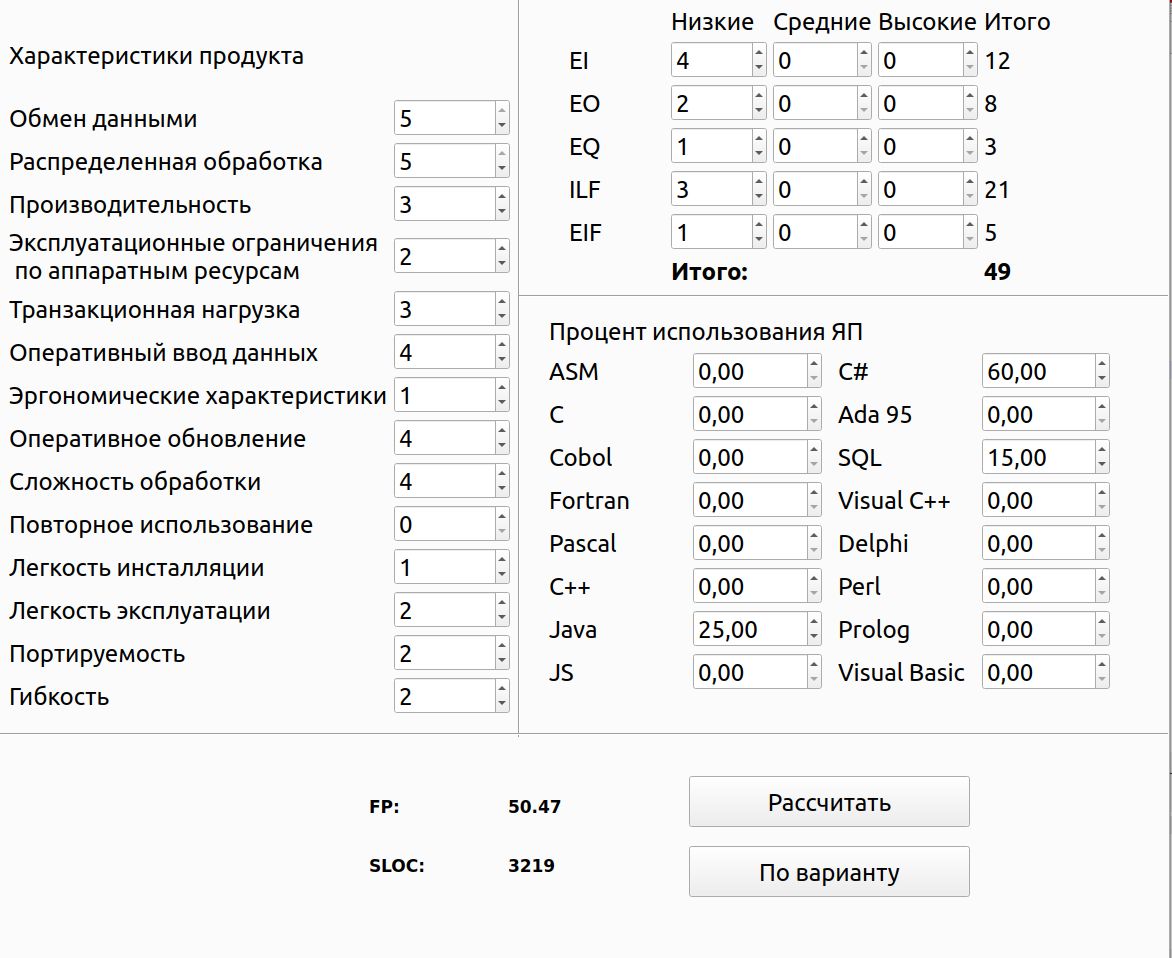
\includegraphics[width=\linewidth]{inc/func.png}
	\end{center}
	\captionsetup{justification=centering}
	\caption{Метод функциональных точек}
\end{figure}
\FloatBarrier 

\anonsection{Расчет показателя степени}
Подберем, исходя из условий, показатели степени, которые нужно использовать для расчета по остальным методам:
\begin{enumerate}
	\item \textbf{Новизна проекта (PREC)} -- почти полное отсутствие прецедентов, в значительной мере непредсказуемый проект.
	\item \textbf{Гибкость процесса разработки (FLEX)} -- по большей части согласованный процесс (график жесткий, точной регламентации нет).
	\item \textbf{Разрешение рисков в архитектуре системы (RESL)} -- некоторое (40\%).
	\item \textbf{Сплоченность команды (TEAM)} -- некоторая согласованность (команда новая, но были проведены определенные мероприятия по сплочению).
	\item \textbf{Уровень развития процесса разработки (PMAT) } -- уровень 1+ (только начинают внедрять).
\end{enumerate}

Итоговый результат: $P = 1.24$.
Результат вычислений представлен на рисунке:
\FloatBarrier
\begin{figure}[h]	
	\begin{center}
		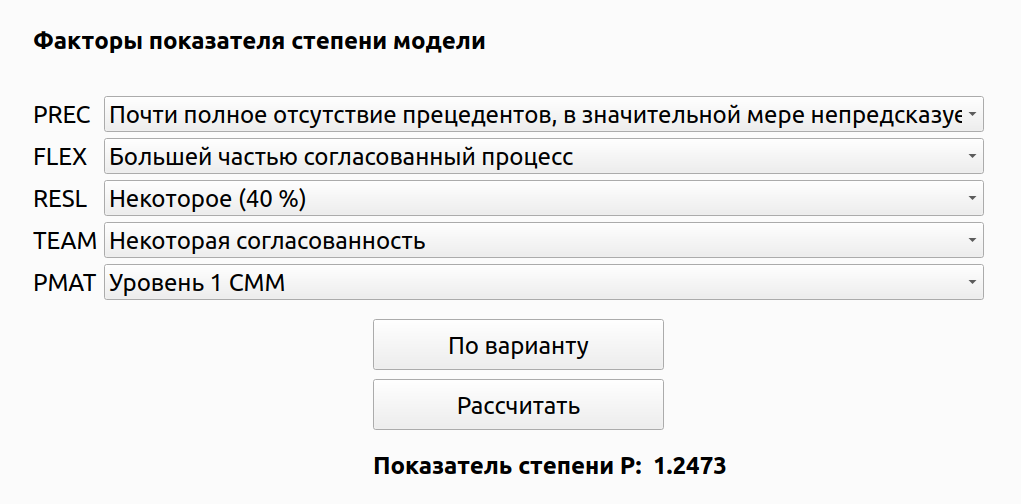
\includegraphics[width=\linewidth]{inc/coef.png}
	\end{center}
	\captionsetup{justification=centering}
	\caption{Расчет показателя степени}
\end{figure}
\FloatBarrier 

\anonsection{Модель ранней разработки архитектуры}
Значение параметров для модели ранней разработки архитектуры были выбраны следующие значения:
\begin{enumerate}
	\item \textbf{PERS} -- номинальный уровень.
	\item \textbf{RCPX} -- очень высокий уровень.
	\item \textbf{RUSE} -- низкий уровень.
	\item \textbf{PDIF} -- высокий уровень.
	\item \textbf{PREX} -- низкий уровень.
	\item \textbf{FCIL} -- высокий уровень.
	\item \textbf{SCED} -- высокий уровень.
\end{enumerate}

Средняя зарплата выбрана 100000 рублей.

Результат вычислений по варианту представлен на рисунке:
\FloatBarrier
\begin{figure}[h]	
	\begin{center}
		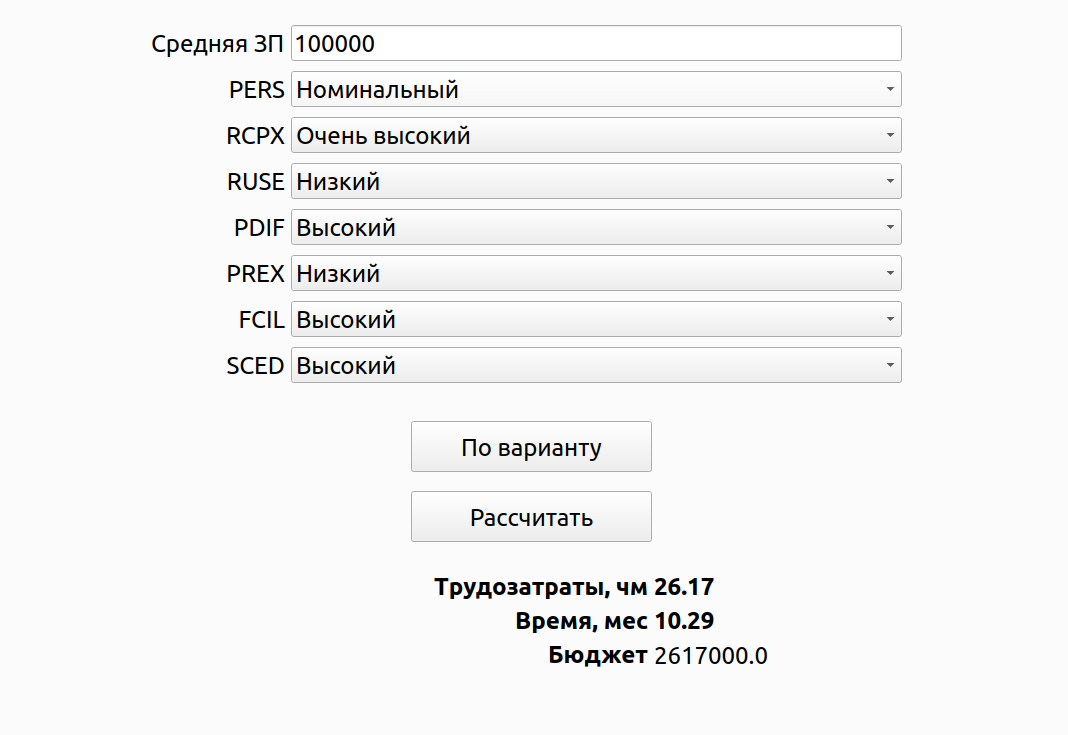
\includegraphics[width=\linewidth]{inc/last.png}
	\end{center}
	\captionsetup{justification=centering}
	\caption{Модель ранней разработки архитектуры}
\end{figure}
\FloatBarrier 

Итоговые результаты:
\begin{itemize}
	\item Требующуюся трудоемкость -- 26.17 человеко-месяц.
	\item Время разработки -- 10.29 месяцев.
	\item Бюджет -- 2617000 рублей.
\end{itemize}

\anonsection{Модель композиции}
Следует определить следующие параметры: 
\begin{enumerate}
	\item RUSE -- 0\%, так как по условию сказано, что повторного использования компонентов не предусматривается.
	\item Средняя зарплата -- 100000 рублей.
	\item Опытность команды -- низкая, так как по условию у персонала низкий опыт разработки систем подобного типа.
	\item Модулей у проекта три -- так как в ТЗ указано, что у реализации будет три компонента.
\end{enumerate}

Экранных форм всего 4.

\begin{itemize}
	\item \textbf{Страница авторизации} -- 3 простых поля и 1 средней сложности (обращение к БД);
	\item \textbf{Страница биржевых сводок} -- 3 простых поля и 1 средней сложности (обращение к БД);
	\item \textbf{Страница заявок} -- 1 простое поле и 2 средней сложности (обращение к БД);
	\item \textbf{Страница новой заявки} -- 4 простых поля и 1 средней сложности (обращение к БД).
\end{itemize}

Из отчетов можно выделить 2 средней сложности: вывод всех заявок и биржевых сводок.

Результат вычислений по варианту представлен на рисунке:
\FloatBarrier
\begin{figure}[h]	
	\begin{center}
		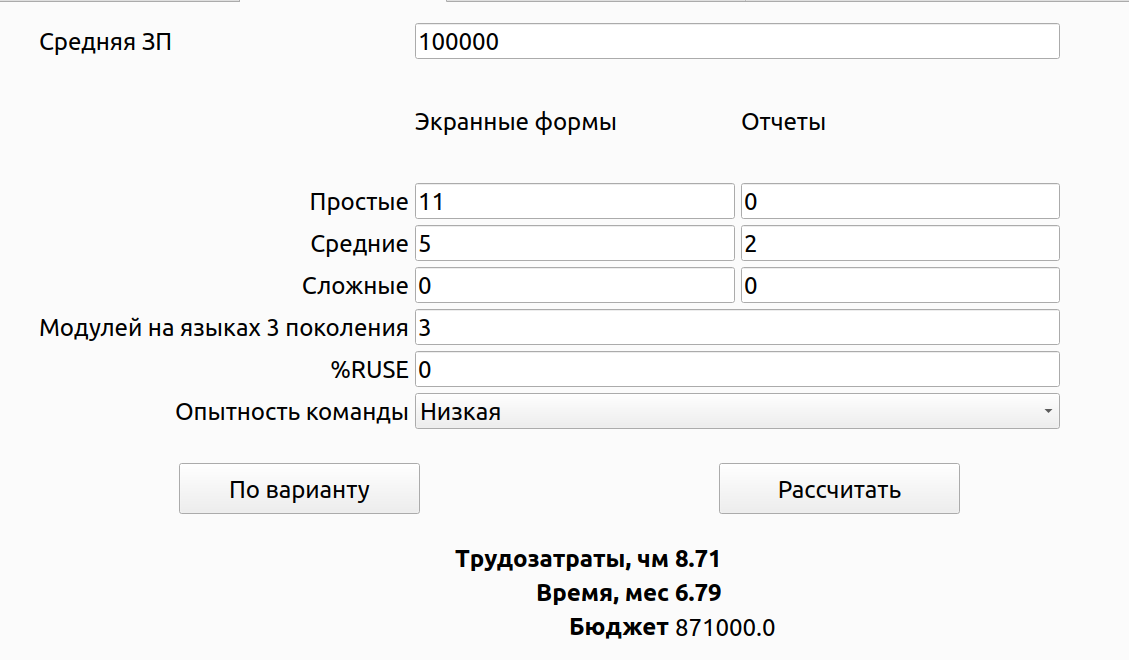
\includegraphics[width=\linewidth]{inc/comp.png}
	\end{center}
	\captionsetup{justification=centering}
	\caption{Модель композиции}
\end{figure}
\FloatBarrier 

Итоговые результаты:
\begin{itemize}
	\item Требующуюся трудоемкость -- 8.71 человеко-месяц.
	\item Время разработки -- 6.79 месяцев.
	\item Бюджет -- 871000 рублей.
\end{itemize}

\anonsection{COCOMO I}
Для выполнения сравнения между моделями требуется проверить результат от модели COCOMO I.

Результат вычислений по варианту представлен на рисунке:
\FloatBarrier
\begin{figure}[h]	
	\begin{center}
		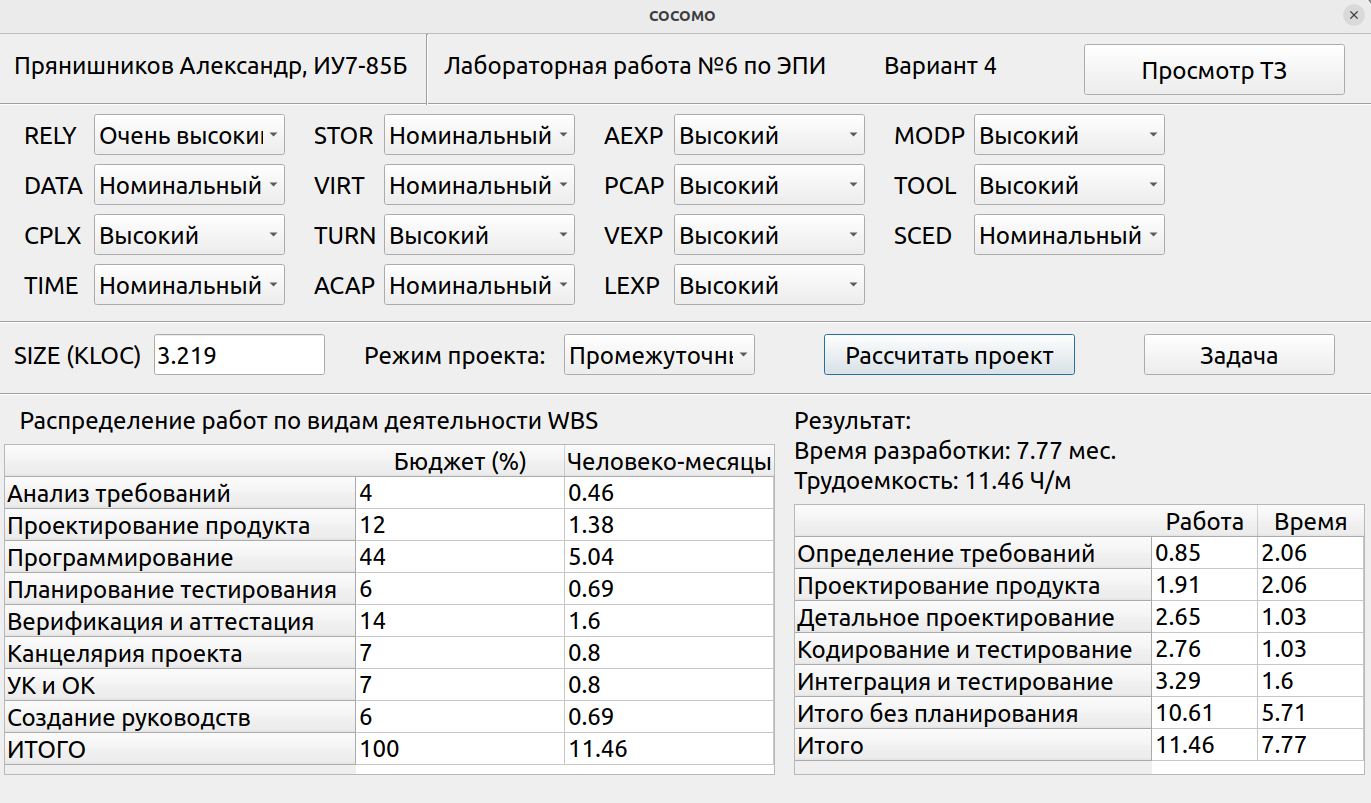
\includegraphics[width=\linewidth]{inc/first.png}
	\end{center}
	\captionsetup{justification=centering}
	\caption{COCOMO I}
\end{figure}
\FloatBarrier 

Итоговые результаты:
\begin{itemize}
	\item Требующуюся трудоемкость -- 11.46 человеко-месяц.
	\item Время разработки -- 7.77 месяцев.
	\item Бюджет -- 1146000 рублей.
\end{itemize}

\anonsection{Выводы}
В качестве моделей для оценки использовалась модель композиции и модель ранней разработки архитектуры.
Выяснилось, что оценка второй модели оказалась по трудозатратам в три раза выше, чем первой -- это связано с более точной оценкой в модели ранней разработки архитектуры. 
В частности, на ее результат влияет метод функциональных точек и более точное разбиение задачей по языкам программирования.

По сравнению с COCOMO I, модель ранней разработки архитектуры увеличивает трудозатраты примерно в два раза, но модель композиции предполагает на 15\% меньше усилий.